\documentclass{article}
\usepackage{fullpage}
\usepackage{indentfirst}
\usepackage{amsmath}
\usepackage{amsfonts}
\usepackage{array}
\usepackage{tipa}
\usepackage{tikz}
\usepackage{tikz-qtree}
\usetikzlibrary{matrix, arrows, automata}
\usepackage{gb4e}
\noautomath
\newcommand{\Y}{$\checkmark$}
\newcommand{\N}{\ding{55}}
\newcommand{\R}{$\Rightarrow$}
\title{Nanjing FST}
\author{Chris Oakden}
\begin{document}
\maketitle
\section{FST on syllable-level representation}
Below is an FST that captures tone sandhi processes in the Nanjing dialect (as ISL functions). Alternations involving checked tones are omitted, and syllable-level representation is used.
\begin{exe}
\ex \label{FST1}
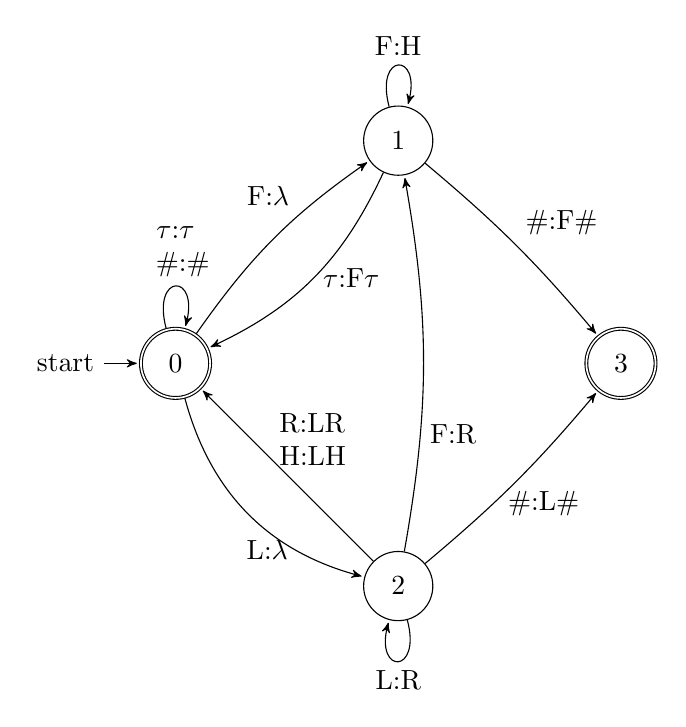
\begin{tikzpicture}[->,>=stealth', shorten >=1pt, auto, node distance = 4cm, baseline = 0]
\node[state,initial, accepting](0){$0$};
\node[state] (1) [above right of=0]{$1$}; 
\node[state] (2) [below right of=0]{$2$};
\node[state, accepting](3) [below right of=1]{$3$};
\path (0) edge [loop above,text width = .5cm, align=center] node {$\tau$:$\tau$ \#:\#} (0);
\path (0) edge [bend left = 10]  node [pos=.65] {F:$\lambda$} (1);
\path (0) edge [bend right] node [below, pos=.6,text width = 1cm, align=center] {L:$\lambda$} (2);
\path (1) edge [loop above] node {F:H} (1);
\path (1) edge [bend left =5] node {\#:F\#} (3);
\path (2) edge [loop below] node {L:R} (2);
\path (2) edge node [above, pos=.5, text width = .2cm, align=center] {R:LR H:LH} (0);
\path (2) edge [bend right =5] node [below, text width=.2cm] {\#:L\#} (3);
\path (1) edge [bend left=20] node [right] {$\tau$:F$\tau$} (0);
\path (2) edge [bend right=10] node [right, pos = .3] {F:R} (1);
\end{tikzpicture}
\end{exe}
Word (or domain) boundaries are included in the representation, as I haven't been able to figure out how to get the ``right-dominant" nature of the patterns within some reference to word boundaries. Transductions on relevant inputs (specifically, lines 1,2,3 and 6 from previous handout (8)) follow. 
\begin{exe}
\ex \label{FFF}
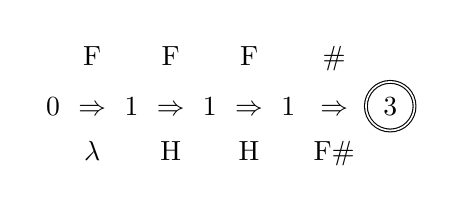
\begin{tikzpicture}[baseline = (m-2-2.base)]
\matrix (m) [matrix of nodes]{
  & F & & F & & F & & \# & \\
0 & $\Rightarrow$ & 1 & $\Rightarrow$ & 1 & $\Rightarrow$ & 1 & $\Rightarrow$ & \node[draw, double, circle]{3}; \\
 & $\lambda$ & & H & & H & & F\# & \\
};
\end{tikzpicture}
\end{exe}
For the string FFF, the machine begins in state 0, taking the F:$\lambda$ transition to state 1 upon reading a F in the input. In intuitive turns, this state is akin to: I have seen a F, if I see another F, I will output a H, otherwise a F. The machine will output transductions on inputs /F$^n$/ for $n$ of any size, as well as string-medial /F$^n$/ sequences. This is guaranteed by the transition $\tau$:F$\tau$ between states 1 and 0 and the looping $\tau$:$\tau$ transition on state 0 (where $\tau$ represents either R or H). \par
The following two example transductions illustrate how the machine incorporates the disyllabic sandhi rules L $\rightarrow$ R / \underline{\hspace{1em}} F and L $\rightarrow$ R / \underline{\hspace{1em}} L.
\begin{exe}
\ex \label{LFF}
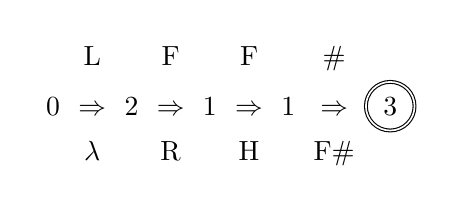
\begin{tikzpicture}[baseline = (m-2-2.base)]
\matrix (m) [matrix of nodes]{
  & L & & F & & F & & \# & \\
0 & $\Rightarrow$ & 2 & $\Rightarrow$ & 1 & $\Rightarrow$ & 1 & $\Rightarrow$ & \node[draw, double, circle]{3}; \\
 & $\lambda$ & & R & & H & & F\# & \\
};
\end{tikzpicture}
\end{exe}
\begin{exe}
\ex \label{LLF}
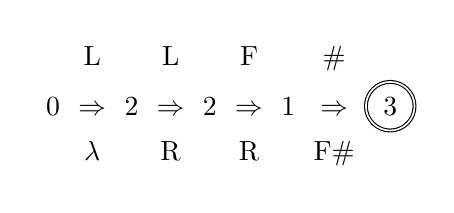
\begin{tikzpicture}[baseline = (m-2-2.base)]
\matrix (m) [matrix of nodes]{
  & L & & L & & F & & \# & \\
0 & $\Rightarrow$ & 2 & $\Rightarrow$ & 2 & $\Rightarrow$ & 1 & $\Rightarrow$ & \node[draw, double, circle]{3}; \\
 & $\lambda$ & & R & & R & & F\# & \\
};
\end{tikzpicture}
\end{exe}
\begin{exe}
\ex \label{LLL}
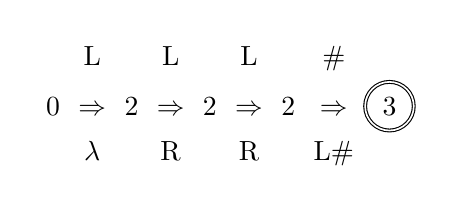
\begin{tikzpicture}[baseline = (m-2-2.base)]
\matrix (m) [matrix of nodes]{
  & L & & L & & L & & \# & \\
0 & $\Rightarrow$ & 2 & $\Rightarrow$ & 2 & $\Rightarrow$ & 2 & $\Rightarrow$ & \node[draw, double, circle]{3}; \\
 & $\lambda$ & & R & & R & & L\# & \\
};
\end{tikzpicture}
\end{exe}
Transductions (\ref{LFF}) - (\ref{LLL}) show that state 2 is L's analog of H's state 1; once a L has been read in the input, the machine waits to read the following symbol to see whether to output a L or R. The cyclic transition L:R captures the canonical ``Mandarin 3rd Tone Sandhi" cases, while the transition F:R to state 1 represents the rule L $\rightarrow$ R / \underline{\hspace{1em}} F. \par
This is a good first run, but it's not perfect. For one, we do not yet have a transition which can account accurately for /$\tau^{n}$FLL$\tau^{n}$/ sequences. Our current machine yields *FLL, since there is no transition from state 1 to state 2. Additionally, state 3 and its transitions are (potentially) superfluous. Since state 0 is an accepting state, we can collapse the \#:F\# and \#:L\# transitions into those which depart from states 1 and 2 (respectively) and terminate in state 0. The FST below shows these changes, highlighted in red.  
\begin{exe}
\ex \label{FST2}
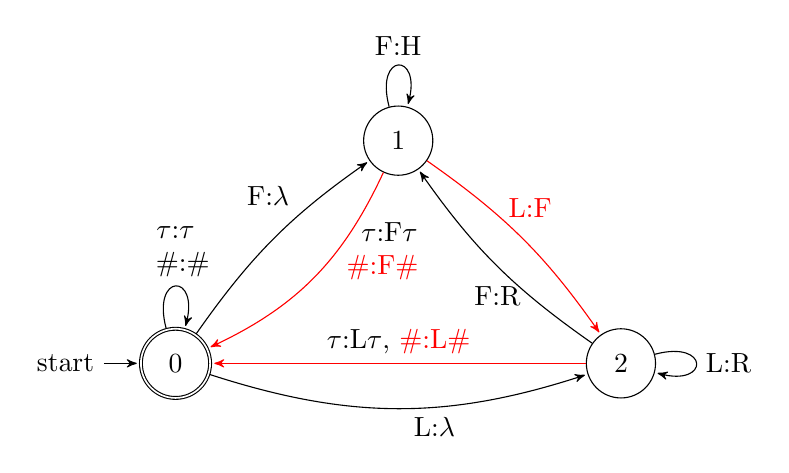
\begin{tikzpicture}[->,>=stealth', shorten >=1pt, auto, node distance = 4cm, baseline = 0]
\node[state,initial, accepting](0){$0$};
\node[state] (1) [above right of=0]{$1$}; 
\node[state] (2) [below right of=1]{$2$};
\path (0) edge [loop above,text width = .5cm, align=center] node {$\tau$:$\tau$ \#:\#} (0);
\path (0) edge [bend left = 10]  node [pos=.65] {F:$\lambda$} (1);
\path (0) edge [bend right=18] node [below, pos=.6,text width = 1cm, align=center] {L:$\lambda$} (2);
\path (1) edge [loop above] node {F:H} (1);
\path (2) edge [loop right] node {L:R} (2);
\path (2) edge [color = red] node [above, pos=.5, text width = 4cm, align=center] {\textcolor{black}{$\tau$:L$\tau$,} \textcolor{red}{\#:L\#}} (0);
\path (1) edge [bend left=20, color = red] node [right, text width = .9cm, align = right, pos = .35] {\textcolor{black}{$\tau$:F$\tau$} \textcolor{red}{\#:F\#}} (0);
\path (2) edge [bend left=10] node [left, pos = .3] {F:R} (1);
\path (1) edge [bend left=10, color = red] node [right, pos = .3, text width = .8cm, align = center] {L:F} (2);
\end{tikzpicture}
\end{exe}
This machine produces the same transductions as (\ref{FFF}) - (\ref{LLL}), with the added benefit of accurate transductions on /$\tau^{n}$FLL$\tau^{n}$/ sequences (as well as being less redundant), as shown below:
\begin{exe}
\ex 
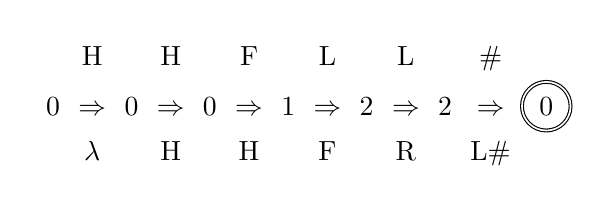
\begin{tikzpicture}[baseline = (m-2-2.base)]
\matrix (m) [matrix of nodes]{
  & H & & H & & F & & L & & L & & \# &  \\
0 & $\Rightarrow$ & 0 & $\Rightarrow$ & 0 & $\Rightarrow$ & 1 & $\Rightarrow$ & 2 & $\Rightarrow$ & 2 & $\Rightarrow$ &  \node[draw, double, circle]{0}; \\
 & $\lambda$ & & H & & H & & F & & R & & L\# \\
};
\end{tikzpicture}
\end{exe}
In the next section, we construct at an FST using melody-tier representations. Will it work?
\section{FST on melodic-tier strings}
Intuitively, translating the FST in (\ref{FST2}) into one that reads symbols on the melodic tier should be straight-forward; some intermediate states will be necessary to capture the fact that two symbols on the melodic tier correspond to a single symbol in syllable-level representation (HL $\equiv$ F; LH $\equiv$ R). The FST below retains the initial state numbers from (\ref{FST2}) and many of its transitions, but adds extra states and transitions with such equivalences in mind.
\begin{exe}
\ex
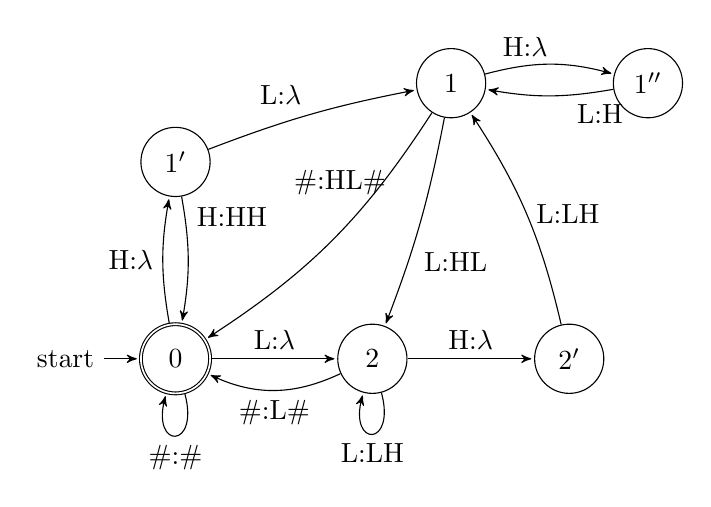
\begin{tikzpicture}[->,>=stealth', shorten >=1pt, auto, node distance = 2.5cm, baseline = 11]
\node[state,initial, accepting](0){$0$};
\node[state] (11) [above of = 0]{$1'$};
\node[state](2) [right of = 0]{2};
\node[state](1)[above of=2, yshift=1cm, xshift=1cm]{1};
\node[state](1'')[right of =1]{$1''$};
\node[state](2')[right of = 2]{$2'$};
\path (0) edge [bend left = 10] node [align=right] {H:$\lambda$} (11);
\path (0) edge node [above] {L:$\lambda$} (2);
\path (0) edge [loop below] node {\#:\#} (0);
\path (11) edge [bend left = 10] node [pos=.3] {H:HH} (0);
\path (11) edge [bend left = 5] node {L:$\lambda$} (1);
\path (1) edge [bend left = 15] node [above, pos = .3] {H:$\lambda$} (1'');
\path (1) edge [bend left = 12] node [left,pos = .25, text width=1cm, align=left] {\#:HL\#} (0);
\path (1) edge [bend left = 5] node[pos = .6] {L:HL} (2);
\path(1'') edge [bend left = 10] node [pos = .35] {L:H} (1);
\path(2) edge [bend left = 25] node [below] {\#:L\#} (0);
\path (2) edge [loop below] node {L:LH} (2);
\path (2) edge node {H:$\lambda$} (2');
\path (2') edge [bend right = 10] node [right] {L:LH} (1);
\end{tikzpicture}
\end{exe}
This machine produces outputs from input strings for trisyllabic sandhi forms using only H and L symbols, and does so accurately (\ref{HLHLHL} - \ref{LLL2}):
\begin{exe}
\ex \label{HLHLHL} /HLHLHL/ $\mapsto$ [HHHL] $\equiv$ /FFF/ $\mapsto$ [HHF] \\
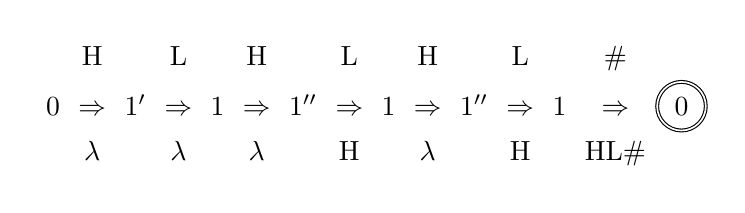
\begin{tikzpicture}[baseline = (m-2-2.base)]
\matrix (m) [matrix of nodes]{
  & H & & L & & H & & L & & H & & L & & \# &  \\
0 & \R & $1'$ & \R & $1$ & \R & $1''$ & \R & 1 & \R & $1''$ & \R & 1 & \R & \node[draw, double, circle]{0}; \\
 & $\lambda$ & & $\lambda$ & & $\lambda$  & & H & & $\lambda$ & & H & &  HL\# \\
};
\end{tikzpicture}
\ex /LHLHL/ $\mapsto$ [LHHHL] $\equiv$ /LFF/ $\mapsto$ [RHF] \\
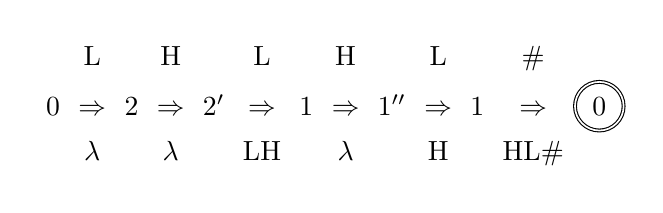
\begin{tikzpicture}[baseline = (m-2-2.base)]
\matrix (m) [matrix of nodes]{
  & L & & H & & L & & H & & L & & \# &  \\
0 & \R & $2$ & \R & $2'$ & \R & $1$ & \R & $1''$ & \R & $1$ & \R & \node[draw, double, circle]{0}; \\
 & $\lambda$ & & $\lambda$ & & LH  & & $\lambda$ & & H & &  HL\# \\
};
\end{tikzpicture}
\ex /LLHL/ $\mapsto$ [LHLHHL] $\equiv$ /LLF/ $\mapsto$ [RRF] \\
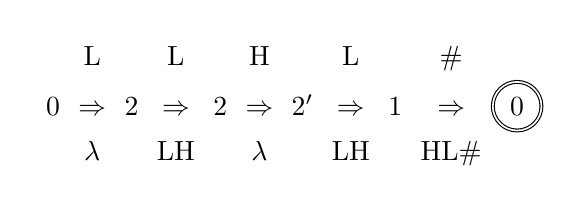
\begin{tikzpicture}[baseline = (m-2-2.base)]
\matrix (m) [matrix of nodes]{
  & L & & L & & H & & L & & \# &  \\
0 & \R & $2$ & \R & 2 & \R & $2'$ & \R & $1$ & \R & \node[draw, double, circle]{0}; \\
 & $\lambda$ & & LH  & & $\lambda$ & & LH & &  HL\# \\
};
\end{tikzpicture}
\ex \label{LLL2} /LLL/ $\mapsto$ [LHLHL] $\equiv$ /LLL/ $\mapsto$ [RRL] \\
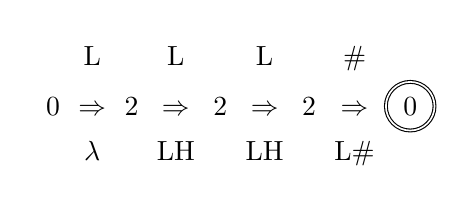
\begin{tikzpicture}[baseline = (m-2-2.base)]
\matrix (m) [matrix of nodes] {
& L & & L & & L & & \# & \\
0 & \R & 2 & \R & 2 & \R & 2 & \R & \node[draw,double,circle]{0}; \\
& $\lambda$ & & LH & & LH & & L\# \\ 
};
\end{tikzpicture}
\end{exe}
A crucial difference between this machine and the machine which accepts syllable-level symbols is that the latter operates over single syllables. Syllable boundaries are thus inherent in single symbols; the number of symbols in a given string will always be equivalent to the number of syllables represented by the string. The same cannot be said of the melody-tier FST given that syllables are represented by either one (H/L) or two (HL/LH) symbols. A given string may have multiple syllabifications, and since the current FST is deterministic, it is bound to produce transductions which do not reflect surface generalizations.
\begin{exe}
\ex
\begin{tabular}[t]{llll}
Input & $\mathtt{cntr(w)}$ & Output & Observed Output \\
\hline
/F.F.F/ & HLHLHL & HHHL & HHHL ($\equiv$ HHF) \\
/H.L.H.L.H.L/ & HLHLHL & *HHHL & HLHLHL \\
/L.F/ & LHL & LHHL & LHHL ($\equiv$ RF) \\
/R.L/ & LHL & *LHHL & LHL
\end{tabular}
\end{exe}
This is reflective of the pitfalls of illicit substructure grammar characterizations of sandhi patterns on the melodic tier. Without adding syllable boundaries to the representation, it is possible to change the transitions on the existing FST to ensure that transductions on the strings above are possible, but the machine loses its determinism as a result (I don't know if we want that). These additional transitions are indicated in red below. Transitions added to create a total function are indicated in blue.
\begin{exe}
\ex
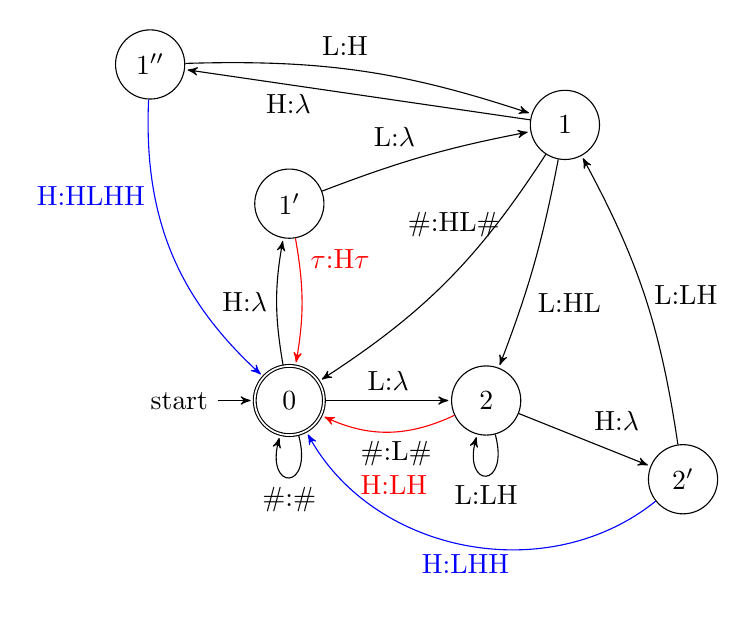
\begin{tikzpicture}[->,>=stealth', shorten >=1pt, auto, node distance = 2.5cm, baseline = 11]
\node[state,initial, accepting](0){$0$};
\node[state] (11) [above of = 0]{$1'$};
\node[state](2) [right of = 0]{2};
\node[state](1)[above of=2, yshift=1cm, xshift=1cm]{1};
\node[state](1'')[above left of =11]{$1''$};
\node[state](2')[right of = 2, yshift=-1cm]{$2'$};
\path (0) edge [bend left = 10] node [align=right] {H:$\lambda$} (11);
\path (0) edge node [above] {L:$\lambda$} (2);
\path (0) edge [loop below] node {\#:\#} (0);
\path (11) edge [color = red, bend left = 10] node [pos=.3] {$\tau$:H$\tau$} (0);
\path (11) edge [bend left = 5] node {L:$\lambda$} (1);
\path (1) edge node [below, pos = .7] {H:$\lambda$} (1'');
\path (1) edge [bend left = 12] node [left,pos = .25, text width=1cm, align=left] {\#:HL\#} (0);
\path (1) edge [bend left = 5] node[pos = .6] {L:HL} (2);
\path(1'') edge [bend left = 10] node [pos = .35] {L:H} (1);
\path(1'') edge [bend right = 25, color = blue] node [pos=.3, left]{H:HLHH} (0);
\path(2) edge [color = red, bend left = 25] node [pos=.5,below, text width = .7cm, align = center] {\textcolor{black}{\#:L\#} \textcolor{red}{H:LH}} (0);
\path (2) edge [loop below] node {L:LH} (2);
\path (2) edge node {H:$\lambda$} (2');
\path (2') edge [bend right = 10] node [right] {L:LH} (1);
\path (2') edge [color = blue, bend left = 50] node [below] {H:LHH} (0);
\end{tikzpicture}
\end{exe}
With these changes, transductions on inputs /H.L.H.L.H.L/ and /R.L/ are no longer problematic.
\begin{exe}
\ex /HLHLHL/ $\mapsto$ [HLHLHL] \\
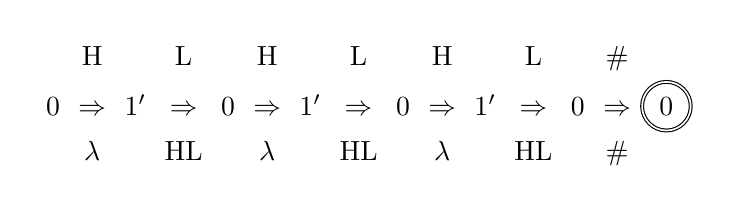
\begin{tikzpicture}[baseline = (m-2-2.base)]
\matrix (m) [matrix of nodes]{
  & H & & L & & H & & L & & H & & L & & \# &  \\
0 & \R & $1'$ & \R & 0 & \R & $1'$ & \R & $0$ & \R & $1'$ & \R & 0 & \R & \node[draw, double, circle]{0}; \\
 & $\lambda$ & & HL  & & $\lambda$ & & HL & & $\lambda$ & & HL & & \# \\
};
\end{tikzpicture}
\ex /LHL/ $\mapsto$ [LHL] \\
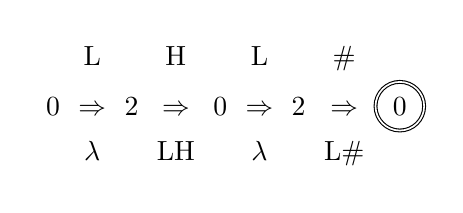
\begin{tikzpicture}[baseline = (m-2-2.base)]
\matrix (m) [matrix of nodes] {
& L & & H & & L & & \# & \\
0 & \R & 2 & \R & 0 & \R & 2 & \R & \node[draw,double,circle]{0}; \\
& $\lambda$ & & LH & & $\lambda$ & & L\# \\ 
};
\end{tikzpicture}
\end{exe}
\end{document}